% Модификатор - команда стиля, действующая, пока не сказано иное (закончится
% область видимости или встретится противоположный модификатор).

\documentclass[a4paper,cmcyralt,12pt]{report}

% КОДИРОВКА И ЛОКАЛИЗАЦИЯ
\usepackage[english,russian]{babel}	% локализация и переносы
\usepackage[utf8]{inputenc} % кодировка исходного кода (input)
\usepackage[T2A]{fontenc} % кодировка выходного текста (output)

% GEOMETRY
\usepackage{geometry}
\geometry{top = 25mm}
\geometry{bottom = 30mm}
\geometry{left = 20mm}
\geometry{right = 20mm}
% Есть и другие параметры (не из пакета geometry):
\linespread{0.7} % междустрочный интервал
\setlength{\parindent}{3ex} % отступ 1-ой строки абзаца
\setlength{\parskip}{2mm} % отступ после начала нового абзаца
% \geometry{paperheight = 297mm}

% КОЛОНТИТУЛЫ
\usepackage{titleps}
\newpagestyle{main}{
  % толщина линии
  \setheadrule{0.4pt}
  % \thepage - номер текущей страницы
  \sethead{лево}{\thepage}{право}
  \setfootrule{5pt}
  \setfoot{лево}{центр}{право}
}
% С этого момента все страницы, если не сказано иное, имеют данный стиль.
\pagestyle{main}

% ШРИФТЫ И НАЧЕРТАНИЯ
\usepackage{soulutf8}

% МАТЕМАТИКА
\usepackage{mathtext} % русские буквы в формулах
\usepackage{amsmath,amsfonts} % математические шрифты
\usepackage{amsthm} % теоремы

% ТЕОРЕМЫ
\theoremstyle{plain}
\newtheorem{theorem}{Моя теорема}
\newtheorem{lemma}{Моя лемма}

% РАЗНОЕ
\usepackage{cmap} % поиск по pdf
\usepackage{hyperref} % кликабельные ссылки
\usepackage{graphicx} % для графики
\usepackage{lipsum} % Lorem ipsum...
\usepackage{alltt} % не игнорирует пробелы
\usepackage{indentfirst} % отступ в начале параграфа

% КАСТОМНЫЕ КОМАНДЫ
% Новая команды с уникальным именем:
\newcommand{\deriv}[2]{\frac{\partial{#1}}{\partial{#2}}}
\newcommand{\R}{\mathbb{R}}
% Переопределение команд (полезно для некоторых греческих букв с непривычными
% очертаниями):
\renewcommand{\phi}{\varphi}
\renewcommand{\epsilon}{\varepsilon}
% Математические операторы (внутри формулы печатаются без курсива и ставят
% пробел перед операндом):
\DeclareMathOperator{\Kerr}{Ker} % так как \Ker может быть занято
% Со "*" создаёт оператор, верхних и нижний индексы которого будут являться
% переделами:
% WARN Не работает для внутристрочных формул!

\DeclareMathOperator*{\argmax}{argmax}
% Бинарные операторы (контролирует расстановку пробелов между операндами):
\newcommand{\rem}{\mathbin{\%}}

% КАСТОМНЫЕ ОКРУЖЕНИЯ
% Имя, что идёт перед содержимым и после:
\newenvironment{centerbf}{\begin{center}\bfseries}{\end{center}}

% ARTICLE
% \title{Название}
% \author{Имя автора}
% \date{\today}
 % подключение файла с преамбулой

\begin{document}

% \maketitle % генерация заголовка, юзает значения параметров, задаваемых
% \title{}, \author{} и \date{} (именно в таком порядке и должны идти заранее)
\input title_example

\tableofcontents % генерация оглавления, юзает только нумерованные разделы
\listoffigures % генерация списка иллюстраций
\listoftables % генерация списка таблиц

\part{Генерируется автоматически}
\chapter{Введение}
\section*{Ненумерованный (не вносится в содержание) раздел}
\subsection[В содержании именуется вот так]{а в тексте вот так (нумеруется как
0-ой)}

% Разделы в порядке убывания значимости:
% part --- часть
% chapter --- глава (отсутствует в article)
% section --- раздел
% subsection --- подраздел
% subsubsection --- подподраздел
% paragraph --- абзац
% subparagraph --- подабзац

% Распознавание символов: \url{https://detexify.kirelabs.org/classify.html}

% Примеры символов, которые надо экранировать: $, \, {}, &, #, _, %

Центрированные формулы лучше писать через экранированные ``[]'', а не ``\$\$''.
А внутристрочные как раз через "\$".

\[
  \int_{- \infty}^{+ \infty} e^{- \frac{x^2}{2}} dx = \sqrt{2 \pi}
\]

\[ \iiiint_{-\infty}^{+\infty} f(x, y, z, w)dxdydzdw = 1 \]

\[ \lim_{n \to \infty} \left( 1 + \frac{1}{n} \right)^n = |t = \frac{1}{n}| = \lim_{t \to +0} \left( 1 + t \right)^\frac{1}{t} = e \]

Во избежание ошибок форматирования надо обрамлять функции без аргументов в
фигурные скобки: {\LaTeX} - наглядный пример.

Фигурные скобки создают область видимости, в которую можно писать модификаторы:
{\bfseries \itshape \Large Жирный курсивный большой}, обычный и {\small
мелкий} текста.

\Huge A
\LARGE A
\Large A
\large A
\normalsize A
\small A

Скобки: (обычные), \big( большие \big), \bigg( огромные \bigg)

Дефисы:
\begin{itemize}
  \item a "--- b \textit{тире для разделения подлежащего и сказуемого}
  \item a --- b \textit{тире}
  \item a -- b \textit{тире для указания числовых промежутков в тексте}
  \item a-b \textit{дефис}
\end{itemize}

% Через \begin{имя окружения}... можно задавать (даже свои) окружения

Пакет \textit{geometry} (./preamble.tex) позволяет настраивать поля и
колонтитулы.
\begin{figure}[h!]
  \centering
  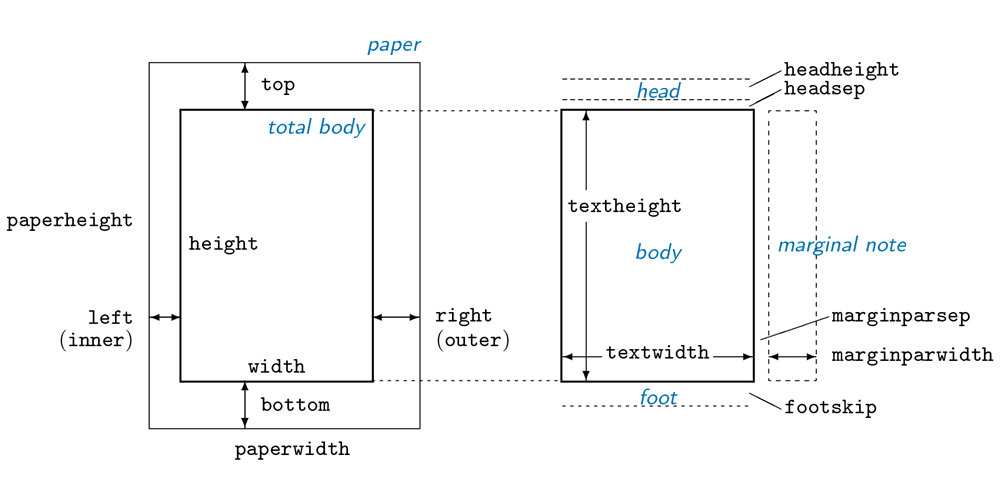
\includegraphics[width=1\textwidth]{./images/geometry.png}
  \caption{geometry}
  \label{figure:geometry}
\end{figure}
% Поддерживаемые единицы измерения:
% pt, ex (высота буквы "x"), em (ширина буквы "M")
% mm (миллиметры), cm (сантиметры), in (дюймы)

% ШРИФТЫ И НАЧЕРТАНИЯ
\so{пробелы между буквами}

\caps{строчные заменяются на ``маленькие'' заглавные}

\ul{подчёркивание}

\st{перечёркивание}

% ОТСТУПЫ

\newpage
Пробел \hspace{1cm} по горизонтали в 1 см

\vspace{2cm}
И по вертикали (сверху) в 2 см

Верх

левый край правый край

% FIXME 
% \vskip

Низ

\newpage

% ТЕОРЕМЫ

Теоремы (./preamble.tex):
\begin{lemma}[Моя лемма]
  \[ 2 + 2 = 2 \times 2 = 2^2 = 4 \]
\end{lemma}

\begin{theorem}[Формула Эйлера]
  \[ e^{i \pi} + 1 = 0 \]
\end{theorem}

\begin{theorem}[Формула площади круга (2-я теорема по счёту)]
  \[ S = 2 \pi r \]
\end{theorem}

\ref{subsect} % кликабельная ссылка на раздел "subsect"

\section{Первый нумерованный раздел}
\subsection{Подраздел}
\label{subsect} % на что ссылается
\subsubsection{Подподраздел (не нумеруется)}

Троеточие\ldots\\
\textbf{Жирный}\\
\textit{Курсив}\\
\underline{Подчёркнутый}\\
Самоучитель: https://www.andreyolegovich.ru/PC/LaTeX.php

\begin{alltt}
  Научный руководитель
  д.ф.-м.н. Бор О.Н.
  Рецензент
  д.ф.-м.н. Басов Н.Г.
\end{alltt}

\begin{itemize}
  \item Маркированный
  \item список
\end{itemize}

\begin{enumerate}
  \item первый пункт
  \item второй
\end{enumerate}

\lipsum[3]\\
\lipsum[2]

% [h!] говорит о том, что мы хотим картинку ИМЕННО в этом месте
\begin{figure}[h!]
  \centering
  \includegraphics[width=1\textwidth]{./images/screw.eps}
  \caption{Винт}
  \label{figure:screw}
\end{figure}

\clearpage % переход к следующей странице, конец той области куда можно вставлять объекты, введенные в код выше

Сверху картинка \ref{figure:screw}

\begin{figure}[h!]
  \centering
  \includegraphics[width=0.1\textwidth]{./images/four_screws.eps}
  \caption{4 винта}
  \label{figure:four_screws}
\end{figure}

% \graphicspath - каталоги (доделать)

\section{Таблицы}
% Доделать

% Данная страница не имеет никакого стиля.
\thispagestyle{empty}

\appendix
\section{Приложение, получается...}
Разделы ниже такой команды будут считаться разделами приложения, со своими
правилами нумерации

\end{document}
